\documentclass{article}

\usepackage{caption}
\usepackage{subcaption}
\usepackage{amsmath}

\usepackage{arxiv}

\usepackage[utf8]{inputenc} % allow utf-8 input
\usepackage[T1]{fontenc}    % use 8-bit T1 fonts
\usepackage{hyperref}       % hyperlinks
\usepackage{url}            % simple URL typesetting
\usepackage{booktabs}       % professional-quality tables
\usepackage{amsfonts}       % blackboard math symbols
\usepackage{nicefrac}       % compact symbols for 1/2, etc.
\usepackage{microtype}      % microtypography
\usepackage{lipsum}
\usepackage{graphicx}

\usepackage{algorithm2e}
\usepackage{authblk}
%\usepackage{bbding}

\usepackage[backend=biber]{biblatex}
\addbibresource{refs.bib}

\graphicspath{ {./fig/} }

\usepackage{tikz}
\usetikzlibrary{arrows.meta, bending, positioning}

\hypersetup{colorlinks=true,linkcolor=blue,filecolor=magenta,urlcolor=cyan}
\newcommand{\map}{\mathop{\bigoplus}\limits}
\newcommand{\txtop}[1]{\mathop{\mathtt{#1}}\limits}

\newcommand{\expr}{\txtop{expression}}

\newcommand{\fn}{\txtop{function}}
\newcommand{\tanhl}{\txtop{tanh}}
\newcommand{\linear}{\txtop{linear}}
\newcommand{\sigmoid}{\txtop{sigmoid}}
\newcommand{\argmin}{\txtop{argmin}}
\newcommand{\einsum}{\txtop{einsum}}
\newcommand{\ntos}{\txtop{noise2self}}
\newcommand{\leiden}{\txtop{leiden}}

\newcommand{\encoder}{\txtop{encoder}}
\newcommand{\decoder}{\txtop{decoder}}
\newcommand{\classifier}{\txtop{classifier}}
\newcommand{\partitioner}{\txtop{partitioner}}

\newcommand{\mathWAK}{\txtop{WAK}}
\newcommand{\mathPWAK}{\txtop{PWAK}}
\newcommand{\mathDEWAKSS}{\txtop{DEWAKSS}}
\newcommand{\mathPart}{\txtop{Partitioner}}
\newcommand{\mathDeePWAK}{\txtop{DeePWAK}}
\newcommand{\mathDeePWAKBlock}{\txtop{DeePWAKBlock}}

\SetKwProg{Fn}{Function}{}{end}
\SetKwProg{Dat}{Data}{}{end}

\SetKwInOut{Hyper}{Hyperparameters}

\SetKwFunction{softmax}{softmax}
\SetKwFunction{MSE}{MSE}
\SetKwFunction{transpose}{transpose}
\SetKwFunction{matmul}{matmul}
\SetKwFunction{eucl}{euclidean}
\SetKwFunction{pca}{pca}
\SetKwFunction{knn}{knn}

\SetKwFunction{sample}{sample}
\SetKwFunction{loss}{loss}
\SetKwFunction{train}{train}

\SetKwFunction{WAK}{WAK}
\SetKwFunction{PWAK}{PWAK}
\SetKwFunction{DEWAKSS}{DEWAKSS}
\SetKwFunction{DeePWAKBlock}{DeePWAKBlock}
\SetKwFunction{DeePWAK}{DeePWAK}

\SetKwFunction{Type}{Type}
\SetKwFunction{List}{List}
\SetKwFunction{Arch}{Arch}
\SetKwFunction{Params}{Params}
\SetKwFunction{Model}{Model}
\SetKwFunction{Linear}{Linear}
\SetKwFunction{Partitioner}{Partitioner}


\date{\today}

\title{Abstracting Features Using Cluster-Embedding Decomposition}
%\title{Sparse Autoencoders, Clustering, and Natural Abstractions}
%\title{Can Sparse Autoencoders Identify Natural Abstractions?}

\author[1]{Keira Wiechecki}
\affil[1]{Center for Genomics \& Systems Biology, New York University,
  \texttt{kaw504@nyu.edu}}

\begin{document}
\maketitle

\begin{abstract}
  I propose a new approach to understanding the feature space of a model based on denoising.
  I further propose that the feature space can be decomposed into two subspaces with intuitive interpretations:
  a cluster space and an embedding space.
  I term this $KE$ decomposition.
  This approach suggests a model's latent ontology can be derived using a paired compressor and a partitioner.
  I present a novel deep clustering architecture based on this principle.
  Preliminary analyses reveal several questions warranting further inquiry.
  
  %Adapting this method to nontrivial models will be involved, but I expect it to represent a substantial advance in interpretability.  
\end{abstract}


\section{Threat Model}

We don't currently know how to specify a \hyperlink{https://arbital.com/p/diamond_maximizer/}{robust goal for a model}.
Because goal space is large, we should expect
\hyperlink{https://www.lesswrong.com/s/r9tYkB2a8Fp4DN8yB/p/FkgsxrGf3QxhfLWHG}{goal misgeneralization as the default outcome}.
We can't currently look inside a model and make any conclusions about its goals.
Mechanistic interpretability (mechinterp) is rapidly improving but is still nowhere near being scalable to frontier models.

To a large extent, deep learning models seem to learn \hyperlink{}{universal} features irrespective of architecture.
This implies the existence of
\hyperlink{https://www.lesswrong.com/posts/gvzW46Z3BsaZsLc25/natural-abstractions-key-claims-theorems-and-critiques-1}{natural abstractions},
which would be a very convenient shortcut for auditing a model.
Unfortunately, the abstractions a model learns seem highly sensitive to choice of training data, and are thus not necessarily universal in the limit.
This means that we cannot expect the abstractions learned by a weak model to remain robust in a more powerful model.

\section{Theory of Change}
\label{sec:2}

\subsection{My macro-scale strategy}
I see the fundamental problems for alleviating this threat as

\begin{enumerate}
  \item formalize the notion of a model's latent concept space
  \item distill a model's latent concept space
  \item enforce decomposability of latent concept space
  \item enforce robustness of existing concepts as the dimensionality of the latent concept space increases
\end{enumerate}

My justification for this line of research is
\begin{enumerate}
\item Almost every alignment proposal is limited by the ability to point at a concept.
\item According to singular learning theory (SLT), any sufficiently parameterized model trained on the same data will converge on the same latent representation of the data.
\item Almost every alignment proposal becomes much more tractable if we can reason about features in isolation.
\end{enumerate}

\subsection{My working theory of ontology}
I refer to any mapping of data to abstractions as an \textit{ontology}.

Rapid progress in scaling LLMs has made it increasingly clear that data rather than compute is the limiting factor on capabilities.
This was not at all obvious in hindsight and if we survive the coming decades it will profoundly reshape every aspect of philosophy.
From an alignment perspective, the universality of deep learning independent of architecture is strong evidence for the natural abstraction hypothesis.
This is very good news! We have evidence that for any given data there is an ``objective'' ground truth.

\subsubsection{Features and concepts}
Mechinterp has been very successful at decomposing models into linear \textit{features}.
Features have proven to be a powerful way of abstracting over activation space.
In other words, mechinterp aims to construct \textit{an ontology of activation space}.

However, this is not the only model ontology we care about.
Many of the concepts humans care about are discrete or stochastic.
For humans, it's unintuitive to think of every image as containing a sliding ``car vector''.
Humans classify images as containing a car.
Note that there is a subtle difference between these two kinds of abstraction.
The former is abstracting over \textit{the pixels in an image} to obtain a characteristic measurement of how ``car'' it is.
The latter is abstracting over \textit{the images in a set} to obtain a likelihood (if we assume differentiability) that the image is in the ``contains car'' category.  
I will refer to the former as \textit{features} and the latter as \textit{concepts}.
If we have some data $X \in \mathbb{R}^{m \times n}$,
where $n$ is the number of samples and $m$ is the number of measurements from each sample, 
features are abstractions over $m$ and concepts are abstractions over $n$.

\subsection{Clustering and latent classification}
I propose that this ``ontology over concepts'' is best expressed in terms of clustering.
Neural networks are continuous, but can learn discrete tasks.
SLT suggests a possible mechanism for this behavior,
but a systematic way of characterizing discretization in the wild remains an open problem.
Though SLT provides a rich thermodynamic description of learning,
an alternative metaphor may be more intuitive.
Consider a latent classifier contained in the model.
Subsequent computations can be conditional on the classification

Additional information on the algorithm are in Appendix \ref{app:bgd}.

%\subsubsection{Empirical abstraction}
%The field of natural abstraction generally deals with the limit behavior of a learning algorithm as data approach infinity.
%I will however restrict my definitions to model training regimes I can run experiments on.
%I refer to the abstractions learned from a specific finite training set as \textit{empirical abstractions}.  
%
%\subsubsection{Denoising, compression, and clustering}
%Ontologies must serve an information theoretic purpose.
%I argue that their primary purpose is minimizing prediction loss through \textit{denoising}.
%Which is to say, discarding information that cannot be used to make inferences.
%I further posit that there are two mechanisms by which ontologies form: compression and clustering.
%These mechanisms are synergistic. Informally, I equate the two with PCA and SVD.
%In my preliminary results, I hope to demonstrate that this intuition has (putative) empirical backing.

\subsection{SAEs and abstraction}
Mechinterp is best charaterized as understanding the abstractions used by a model.
\hyperlink{}{Sparse autoencoders} (SAEs) have become a powerful tool for identifying monosemantic features.
Though SAE features are significantly more interpretable than raw activations, interpreting them is still a daunting task.
\hyperlink{https://www.lesswrong.com/posts/f9EgfLSurAiqRJySD/open-source-sparse-autoencoders-for-all-residual-stream}{A high quality library for a single layer}
can contain over 25,000 features.
It would be a substantial interpretability advance if we could impose structure on these features.

Existing research on SAEs suggests that features assemble into clusters representing higher order features.
This suggests the possibility of a hierarchical organization of features.
Characterizing features requires carefully balancing feature sparcity and accurately reconstructing the model activations.
We would like to be able to selectively zoom in on features.



%\begin{multicols}{2}

\section{Plan}

\subsection{Current Research Questions}
\begin{enumerate}
    \item Can a PSAE recover latent classifications from a toy model?
    \item Can PSAEs be used to aggregate SAE features?
    \item Are PSAE features more interpretable than SAE features?
    \item Can interpretability of a feature be defined in terms of effective information?
    \item Can we define a proxy metric for interpretability based on feature perturbation?
    \item Are cluster centroids from a PSAE representative of ``central cases'' of a classification?
    \item Can a PSAE detect formation of concepts during training?
    \item How does this compare to devinterp SOTA?
    \item Can PSAE clusters be used as a proxy for effective information gain during training?
\end{enumerate}

\subsection{Further Research Questions}
\begin{enumerate}
    \item How do linear combinations of PSAEs behave?
    \item How do sequential PSAEs differ from parallel PSAEs?
\end{enumerate}

\subsection{Big Questions}
\begin{enumerate}
    \item Is effective information a useful measure of model capability?
    \item Is it possible to have a model-independent measure of effective information of a data set?
    \item Are PSAEs a fully general clustering solution?
    \item Can a metaontology be expressed in terms of PSAEs?
\end{enumerate}

\begin{figure}
    \centering
     %\begin{subfigure}[b]{0.5\textwidth}
        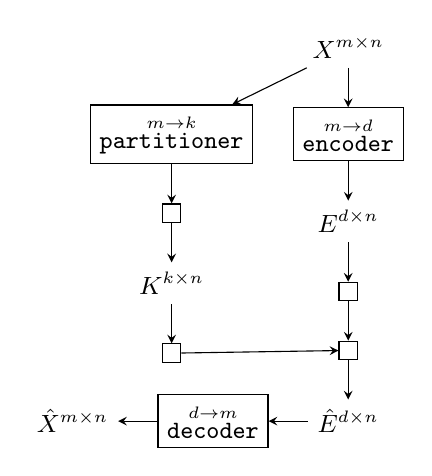
\begin{tikzpicture}[
    node distance = 5mm and 5mm,
    punkt/.style = {rectangle, draw},
    pil/.style = {black, -stealth},
    font=\small
    ]

  %\node[punkt] (preprocessing) {preprocessing} ;
  \node[] (X) {$X^{m \times n}$} ;
  \node[punkt] (encoder) [below=of X] {$\encoder^{m \to d}$} ;
  \node[] (E) [below=of encoder] {$E^{d \times n}$} ;
  \node[punkt] (Etranspose) [below=of E] {\transpose} ;

  \node[punkt] (partitioner) [left=of encoder] {$\partitioner^{m \to k}$} ;
  \node[punkt] (softmax) [below=of partitioner] {\softmax} ;

  \node[] (K) [below=of softmax] {$K^{k \times n}$} ;
  %\node[punkt] (Ktranspose) [left=of K] {\transpose} ;
  %\node[punkt] (KK) [below=of Ktranspose] {\matmul} ;
  %\node[] (P) [below=of KK] {$P^{n \times n}$} ;
  \node[punkt] (wak) [below=of K] {\PWAK} ;
  \node[punkt] (GE) [below=of Etranspose] {\matmul} ;
  \node[] (Ehat) [below=of GE] {$\hat{E}^{d \times n}$} ;

  \node[punkt] (decoder) [left=of Ehat] {$\decoder^{d \to m}$} ;
  \node[] (Xhat) [left=of decoder] {$\hat{X}^{m \times n}$} ;

  \draw[pil] %(preprocessing) edge (X)
  (X) edge (encoder)
  (encoder) edge (E)
  (E) edge (Etranspose)
  (Etranspose) edge (GE)
  
  (X) edge (partitioner)
  (partitioner) edge (softmax)
  (softmax) edge (K)
  (K) edge (wak)
  %(Ktranspose) edge (KK)
  %(K) edge (KK)
  %(KK) edge (P)
  %(P) edge (wak)
  (wak) edge (GE)
  (GE) edge (Ehat)

  (Ehat) edge (decoder)
  (decoder) edge (Xhat);
\end{tikzpicture}


      %   \caption{}
      %   \label{fig:}
     %\end{subfigure}
     %\hfill
     
     \caption{
     $KE$ decomposition forward pass. 
     $E_{outer}$ is the activation matrix obtained from an outer model.
     For $n$ samples with $m$ activations, an inner encoder embeds each as a vector of length $d$.
     An inner classifier assigns probabilities for each sample being in each of $k$ clusters.
     Using the \PWAK transformation (see Appendix \ref{app:pwak}), 
     we obtain a denoising diffusion kernel based on the probability of sample pairs being in the same cluster.
     Matrix multiplication of the kernel with the inner embeddings gives denoised embeddings.
     The decoder unembeds the denoised embeddings back into activations of the outer model.
     The general method can be combined with any inner encoder, decoder, and classifier.
     See Appendix \ref{app:notation} for notation details.
     }
     \label{fig:deepwak}
\end{figure}

\subsection{Immediate goals}
\secsubhead{2-3 weeks}
\begin{enumerate}
    \item Train a toy model of feature splitting with checkpoints
    \item Implement an SAE and PSAE for the toy model
    \item Measure change in effective information during training
    \item Implement feature visualization
    \item Causal intervention on features
\end{enumerate}

\subsection{Initial paper}
\secsubhead{5 weeks}
\begin{enumerate}
    \item Review literature on interpretability metrics
    \item Determine how to quantify the interpretability of a feature
    \item Gain a better understanding of how causal emergence and SLT fit together
    \item Document git repo
    \item Separate writeup on theory \& how it fits into a broader alignment agenda
\end{enumerate}

\subsection{Medium term goals}
\secsubhead{4 months}
\begin{enumerate}
    \item Investigate bisemanticity: can we reconstruct a latent decision tree?
    \cite{aytekin2022neural}
    \item Adapt PSAE to GPT-2
    \item Determine if PSAE features contain more effective information than SAE features
    \item Compare effective information to techniques from 
    existing literature on developmental stages\cite{hoogland2024developmental}
\end{enumerate}

\subsection{6 month goals}
\begin{enumerate}
    \item Performance optimization
    \item Code distribution
    \item Toy model of illusory interpretability
    \item Develop metric for ``patchability'' of features
    \item Determine if ``patchability'' is a useful proxy for interpretability
\end{enumerate}

\subsection{1 year goals}
\begin{enumerate}
    \item Develop a toy model for learning an ontology
    \item Develop quality metrics for an ontology
    \item Test ontologizer architectures
\end{enumerate}

\subsection{Evaluation}

\paragraph{Cluster enrichment}
I perform a \hyperlink{https://en.wikipedia.org/wiki/Hypergeometric_distribution#Hypergeometric_test}{hypergeometric test}
for pairwise enrichment of all classifications in each model (Fig. \ref{fig:hyperMNIST}.
Clusters should correspond to the classifications of the outer model.

\paragraph{Effective information gain}
Clusters should become more degenerate over the course of (outer model) training.

\paragraph{Causal intervention}
How does perturbing a feature affect model behavior?
Is it easier to elicit desired behavior from PSAE features?

\paragraph{Adversarial activation patching}
Is it \textit{harder} to produce illusory interpretability by intervening on PSAE features?
It may be relevant that PSAE tends to produce fewer ``dead'' features (Fig. \ref{fig:E_MNIST}

\paragraph{Visual inspection}
Do cluster centroids correspond to recognizable features?

\subsection{Progress}
I attempt to determine whether an autoencoder combined with a self-supervised classifier produces more interpretable features than a na\"ive SAE.
I perform clustering with multiple architecture variants to assess stability of the latent classifications.
I try to assess whether a toy model trained on the same data but with different objectives learns the same abstractions.

\subsubsection{My toy model of feature splitting}
I trained a MNIST classifier with a 3 neuron bottleneck.
I hypothesized that since the model had more labels than neurons in the bottleneck, features would be represented in superposition.
I refer to this as the ``outer model''.
Details are in Appendix \ref{app:outer}.

%\subsection{Feature splitting}
I train three ``inner models'' to split the bottleneck activations into sparse features.
One is a canonical SAE. 
The others are variants on the architecture depicted in Fig. \ref{fig:deepwak}.
Details are in Appendix \ref{app:inner}.

See Appendix \ref{app:progress} for progress checklists.

%\end{multicols}

%\begin{multicols}{2}
\section{Preliminary Results}
\secsubhead{I apologise for the information density of the figures.
I didn't have time to make simpler ones.}
\label{app:results}

\subsection{How to read the figures}
\label{sec:heatmaps}
%Heatmaps are ubiquitous in bioinformatics for visualizing very large data sets.
In Fig. \ref{fig:E_MNIST} and \ref{fig:K_MNIST}, rows are samples and columns are activations.
Samples are split either by training label (Fig. \ref{fig:E_MNIST}) or predicted label (Fig. \ref{fig:K_MNIST}.
Activations are split by model.
For Fig. \ref{fig:E_MNIST}, these are the encoder activations.
\textsf{bottleneck} gives the bottleneck activations for the outer model.
%\end{multicols}

\begin{figure}{\textwidth}
\centering
\includegraphics[width=\textwidth]{fig/loss_outer.pdf}
\caption{Outer model loss (logit crossentropy) compared to data labels.}
\label{fig:lossouter}
\end{figure}

\begin{figure}{\textwidth}
    \centering
    \includegraphics[width=\textwidth]{fig/loss_inner.pdf}
    \caption{Inner model loss (logit crossentropy) compared to the prediction of the outer model.}
    \label{fig:lossinner}
\end{figure}


\begin{figure}
  \includegraphics[width=\textwidth]{E_labels.pdf}
  \caption{Feature splitting of bottleneck activations by different methods.
    There is a clear progression of sparcity from a na\"ive SAE, PSAE, and DeePWAK.
    Rows are split by training set label.
    Interestingly, adding a partitioner submodel seems to result in the same feature being copied by multiple embeddings.}
    \label{fig:E_MNIST}
\end{figure}

\begin{figure}
  \includegraphics[width=\textwidth]{K_predicted.pdf}
    \caption{Both DeePWAK and PSEA learn sparse clusters. Rows are split by predicted label.}
    \label{fig:K_MNIST}
\end{figure}

\begin{figure}
  \includegraphics[width=\textwidth]{enrichment.pdf}
    \caption{Hypergeometric test for enrichment of [rows] in [columns].}
    \label{fig:hyperMNIST}
\end{figure}

%\begin{multicols}{2}
    
Even trained without a sparcity correction, \DeePWAK finds a more sparse representation than the SAE or PSAE (Fig. \ref{fig:E_MNIST}, \ref{fig:K_MNIST}.

Both DeePWAK and PSAE seem to capture latent features from the bottleneck (Fig. \ref{fig:hyperMNIST}.
Strikingly, PSAE better predicts the model output than the model predicts the training labels.
DeePWAK, on the other hand, appears to identify higher level features used by the model for classification.
It reveals the model apparently grouping rounded (0,3,6,8) and pointed (4,5,7,9) digits. 
Even more curiously, these features appear \textit{bisemantic}.
Looking at \textsf{DeePWAK 0}, this cluster appears to regard 6 as ``opposite'' of 1.
If we look back at Fig. \ref{fig:K_MNIST}, we can see the partitioner is much less confident classifying 6s than other digits.
It's possible the model is using an internal logic of ``I don't know what this is but it's definitely not a 1''.




\printbibliography

\appendix

\section{Notation}
\label{app:notation}
We use lowecase Latin characters to denote scalars, boldface lowecase characters to denote vectors, and capital Latin characters to denote matrices.
Subscripts indicate indices.
Because we will mostly be working with matrices in $\mathbb{R}$, we abbreviate $X : \mathbb{R}^{m \times n}$ as $X^{m \times n}$.
We use a circumflex to indicate a reconstruction of an input by a predictor.
Lowercase Greek characters indicate the parameters of a model.
Capital Greek letters indicate parameter spaces.
Function names are in monospace.

$\fn^{n \to m}$ indicates a layer with input dimension $n$, output dimension $m$, and activation function $\fn$.

\section{Additional Background}
\label{app:bgd}

\subsection{Denoising the data explains the data}
\label{app:ntos}
For a large class of denoising functions, it is possible to find optimal parameters using only unlabeled noisy data\cite{batson2019noise2self}.
$\ntos$ gives a near-maximally-general optimization target for hyperparameter search.


Let $J \in \mathcal{J}$ be independent partitions of noisy data $X$.
Let $\mathcal{F}(\theta)$ be a family of predictors of $X_J$ with tunable parameters
$\theta \in \Theta$ that depends on its complement $X_{J^C}$

\begin{equation}
  \hat{X}_J=\mathcal{F}(\theta)(X_{J^C})
\end{equation}

In other words, $\mathcal{F}$ predicts each data point $X_J$ from some subset of the data excluding $X_J$. 

  The optimal $\theta$ is given by

\begin{equation}
  \label{eq:ntos}
  \ntos_\theta^{\Theta}[\mathcal{F}(\theta),X] := \argmin_\theta^{\Theta}[\sum_{J}^{\mathcal{J}}\mathbb{E}[X_J-\mathcal{F}(\theta)(X_{J^C})]^2]
\end{equation}

\subsection{Diffusion with weighted affinity kernels}

$\ntos$ is particularly useful for finding optimal parameters for generating a graph\cite{tjarnberg2021}.
(see Appendix \ref{app:DEWAKSS})
The adjacency matrix $G$ of any graph can be treated as a transition matrix (or weighted affinity kernel) by setting the diagonal to 0 and normalizing columns to sum to 1. We call this the \WAK function (Algorithm \ref{alg:WAK}).

For each value in data $X$, an estimate is calculated based on its neighbors in the graph. This can be expressed as matrix multiplication.

\begin{equation}
  \label{eq:WAK}
\hat{X} := \WAK(G)X^\top
\end{equation}


\subsection{Partitioned weighted affinity kernels} 
\label{app:pwak}

Though DEWAKSS uses a $k$-NN graph, any adjacency matrix will do.
A clustering can be expressed as a graph where points within a cluster are completely connected and clusters are disconnected.

Let $K^{k \times n}$ be a matrix representing a clustering of $n$ points into $k$ clusters. Let each column be a 1-hot encoding of a cluster assignment for each point. We can obtain a partition matrix $P \in \mathbb{R}^{n \times n}$ by what we'll call the \textit{partitioned weighted affinity kernel} (\PWAK) function.

\begin{equation}
  \label{eq:PWAK}
  \PWAK(K) := \WAK(K^\top K)
\end{equation}

This lets us define a loss function

\begin{equation}
  \mathcal{L}_{\mathPWAK}(K,X) := \mathbb{E}[\mathPWAK(K)X^\top - X]^2
\end{equation}


\PWAK can be extended to soft cluster assignment, making it possible to learn $K$ via SGD.
We will refer to a model of this sort as a \Partitioner to emphasize that while it returns logits corresponding to classifications, there are no labels on the training data.

There is no accuracy measure separate from the decoder loss.
The partitioner simply tries to find the best $P$ for minimizing loss of the decoded output.

The only hyperparameters are the maximum number of clusters, the neural net architecture, and the training hyperparameters.
Because $PX^\top$ is $\mathcal{J}$-invariant, this classifier will converge on a solution less than the maximum $k$.
Intuitions from transformers may be helpful in visualizing why this works.
Informally, $P$ can be equated to position-independent attention with data points as tokens and the batch size as the context window.
Attentive readers may make a connection between masking the diagonal and BERT.

We can now train a model to classify unlabeled data into an undefined number of clusters with no prior distribution in $\mathcal{O}(n^2)$ time!


\end{document}
